\section{Conventional analysis}

  I have decided to conduct a conventional analysis to check whether we can find some regularities or anomalies that will help identifying groups of users using non-complex network methods.
  
  \subsection{Time oriented distribution of posts}
  
    First, I decided to have a look at the distribution of messages in topics during each year, month and hour during the day. The forum started in June 2001 and has had successively more messages posted per year for 6 consecutive years. Then it suddenly stopped and noted a significant, 32.36\% drop in message count in 2008. In this year, the United States of America, as well as pretty much the rest of the World, has suffered from major financial crisis. I never had access to the information about the \emph{page views}\footnote{Individual page impressions happening when users browse the website} of this particular message board, but I suspect that it might have been one of the reasons why an interest of the forum specialised in somewhat expensive equipment has decreased during that time. Figure \ref{fig:dist_year} shows the number of messages posted during each year of the data I have gathered (from June 21, 2006 to April 10, 2012).
    
    \begin{figure}[H]
      \centering
      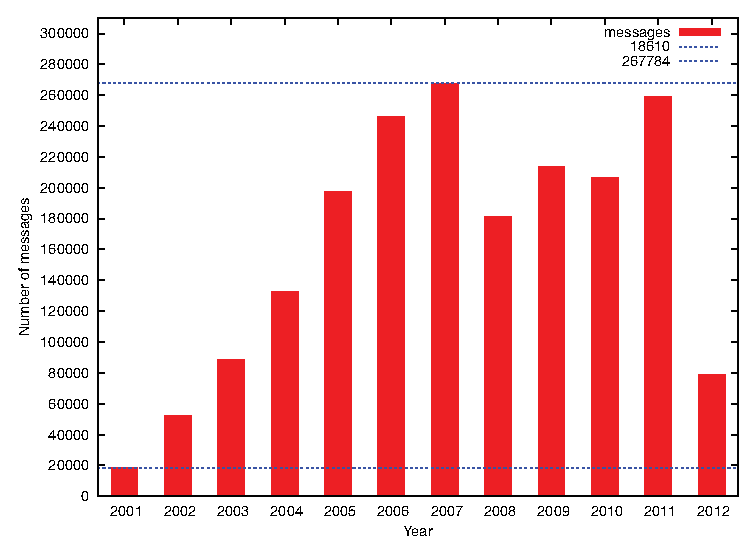
\includegraphics[width=\textwidth]{chapters/03_implementation/yearly}
      \caption{Message number distribution by year}
      \label{fig:dist_year}
    \end{figure}
    
    Out of the curiosity I wanted to find out if I can confirm my suspicions by plotting the number of words related to prices against the total number of words. Figures \ref{fig:dist_price_year_1} and \ref{fig:dist_price_year_1} exhibit this ratio: the former, shown in full scale, and the latter \textquote{zoomed in} to exaggerate the peak usage that has happened during the year 2009. It may or may not be related to the Great Recession of 2009\footnote{D. Wessel from The Wall Street Journal (2010-04-08). \emph{Did \textquote{Great Recession} Live Up to the Name?} (available at http://online.wsj.com/article/SB10001424052702303591204575169693166352882.html) \\ C. Rampell from New York Times (2009-03-11). \emph{\textquote{Great Recession}: A Brief Etymology.} (available at http://economix.blogs.nytimes.com/2009/03/11/great-recession-a-brief-etymology/)} following the financial crisis of 2008. I will not follow on this topic any longer since this thesis is not about interpretation of the data from an economic standpoint.
    \begin{figure}[H]
      \centering
      \begin{subfigure}[H]{0.7\textwidth}
        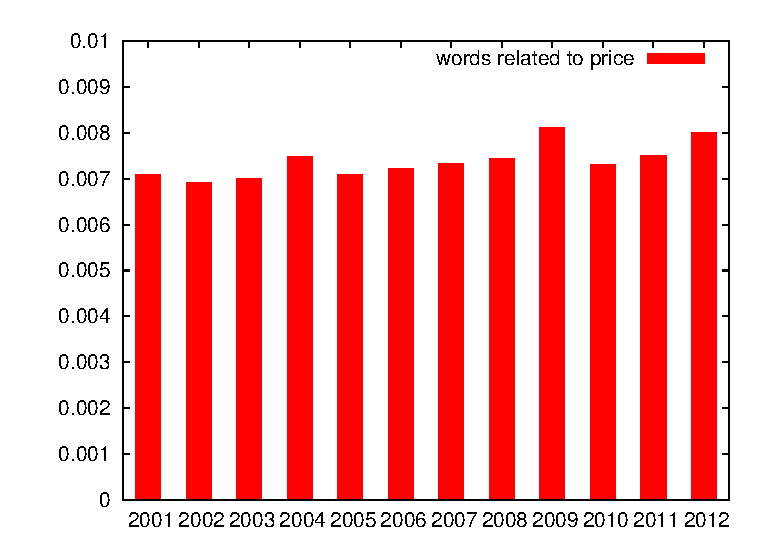
\includegraphics[width=\textwidth]{chapters/03_implementation/yearly_price1}
        \caption{Full scale}
        \label{fig:dist_price_year_1}
      \end{subfigure}
      \\
      \begin{subfigure}[H]{0.7\textwidth}
        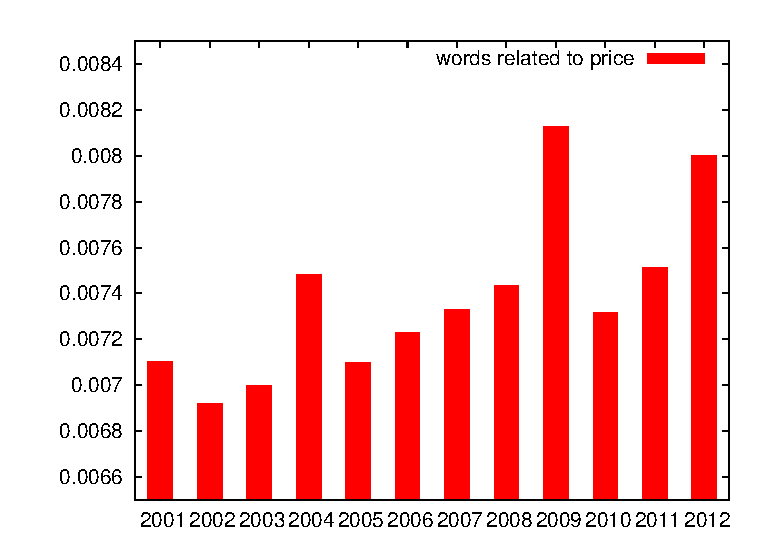
\includegraphics[width=\textwidth]{chapters/03_implementation/yearly_price2}
        \caption{Scale zoomed in}
        \label{fig:dist_price_year_2}
      \end{subfigure}
      \caption{Ratio of the usage of words related to prices to the total number of words}
      \label{fig:dist_price_year}
    \end{figure}
    
    Test
    
    \begin{figure}[H]
      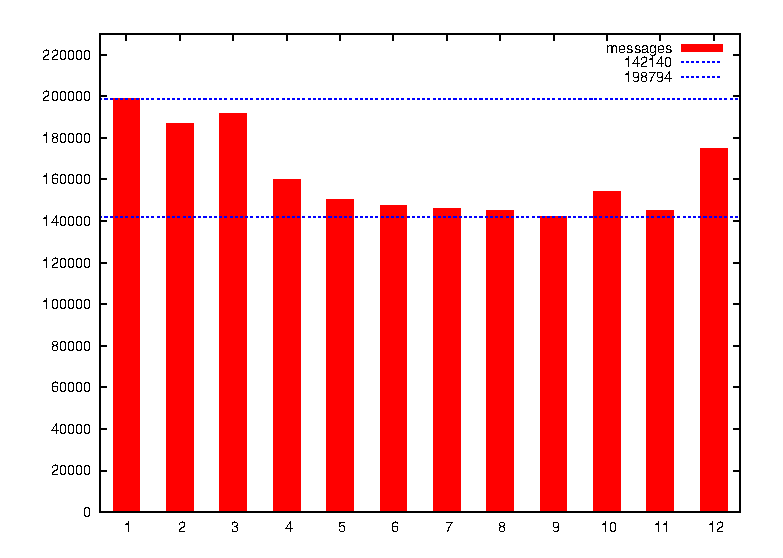
\includegraphics[width=\textwidth]{chapters/03_implementation/monthly}
      \caption{Message number distribution by month}
      \label{fig:dist_month}
    \end{figure}
    
    \begin{figure}[H]
      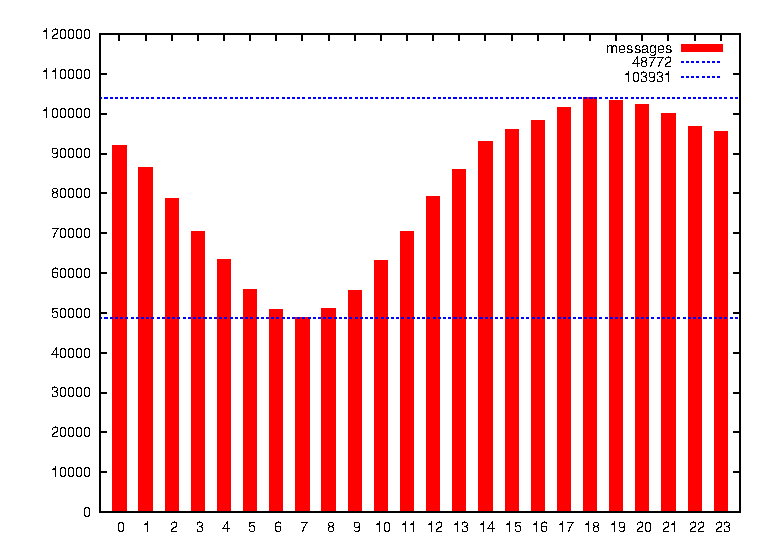
\includegraphics[width=\textwidth]{chapters/03_implementation/hourly}
      \caption{Message number distribution by hour}
      \label{fig:dist_hour}
    \end{figure}